\documentclass[14pt,a4paper]{extarticle}
\usepackage[T1]{fontenc}
\usepackage[utf8]{inputenc}
\usepackage[scaled]{helvet}
\renewcommand{\familydefault}{\sfdefault}
\usepackage{amsmath}
\usepackage{sansmath}
\sansmath
\usepackage[a4paper,margin=2cm]{geometry}
\usepackage{tikz}
\usetikzlibrary{angles,quotes,patterns}
\usepackage{array}
\pagestyle{empty}
% Zweite Seite: 5-mm-Kästchen, 1 cm Rand
\newcommand{\kaestchen}{\newpage\null
\begin{tikzpicture}[remember picture,overlay]
\begin{scope}[shift={(current page.south west)}]\draw[step=5mm, black!45, line width=0.3pt] (1cm,1cm) grid (20cm,28.5cm);\draw[black!45, line width=0.3pt] (1cm,1cm) rectangle (20cm,28.5cm);\end{scope}
\end{tikzpicture}}
\setlength{\parindent}{0pt}
\hyphenpenalty=10000

% Nur Schwarz und Grau, die Blätter werden schwarz-weiß kopiert.
% Merkblock: Begriff und Text links, Zeichnung rechts.
\newcommand{\bl}{0.5}
\newcommand{\block}[3]{%
\begin{minipage}[c]{\bl\textwidth}\raggedright{\Large\bfseries #1\par}\medskip #2\end{minipage}\hfill
\begin{minipage}[c]{\dimexpr0.97\textwidth-\bl\textwidth\relax}\centering #3\end{minipage}\par}

\renewcommand{\bl}{0.46}
\begin{document}

{\LARGE\bfseries Umkreis und Inkreis\par}
\vspace{0.9cm}

\block{Umkreis}{%
Der Umkreis geht durch alle drei Ecken. Sein Mittelpunkt $U$ ist der Schnittpunkt der Mittelsenkrechten. $U$ ist von allen Ecken gleich weit entfernt.\par\medskip
\begin{tabular}{@{}l@{\ }>{\raggedright\arraybackslash}p{0.88\linewidth}@{}}
1. & Mittelsenkrechten von zwei Seiten zeichnen\\
2. & Ihr Schnittpunkt ist $U$\\
3. & Kreis um $U$ durch eine Ecke
\end{tabular}\par\medskip
Hat das Dreieck einen stumpfen Winkel, liegt $U$ außerhalb.}{%
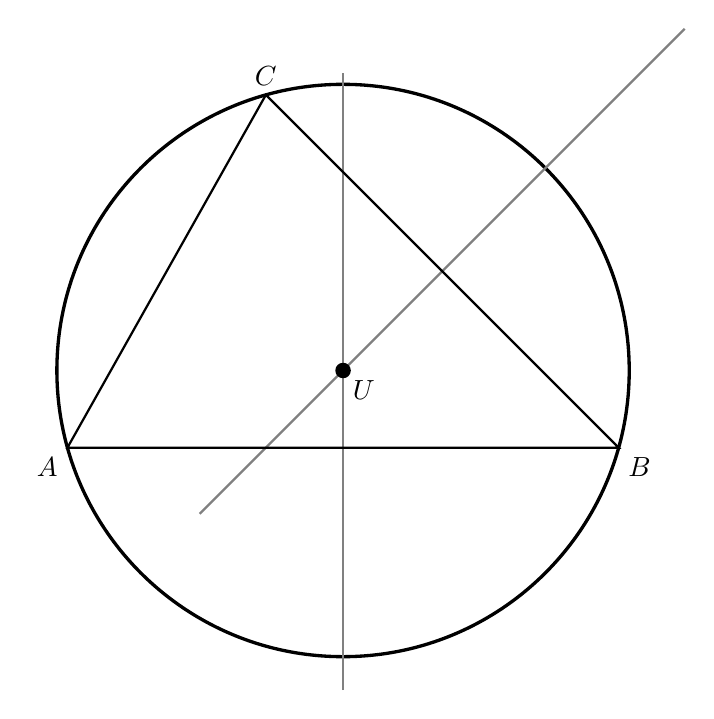
\begin{tikzpicture}[scale=1.4]
  \coordinate (A) at (0,0); \coordinate (B) at (5,0); \coordinate (C) at (1.8,3.2); \coordinate (U) at (2.5,0.7);
  \draw[very thick] (U) circle (2.596);
  \draw[gray, thick] (2.5,-2.2) -- (2.5,3.4);
  \draw[gray, thick] (3.4,1.6) ++(-2.2,-2.2) -- ++(4.4,4.4);
  \draw[thick] (A) -- (B) -- (C) -- cycle;
  \fill (U) circle (2pt) node[below right] {$U$};
  \node[below left] at (A) {$A$}; \node[below right] at (B) {$B$}; \node[above] at (C) {$C$};
\end{tikzpicture}}

\vspace{1cm}

\block{Inkreis}{%
Der Inkreis berührt alle drei Seiten. Sein Mittelpunkt $W$ ist der Schnittpunkt der Winkelhalbierenden. $W$ ist von allen Seiten gleich weit entfernt.\par\medskip
\begin{tabular}{@{}l@{\ }>{\raggedright\arraybackslash}p{0.88\linewidth}@{}}
1. & Winkelhalbierende von zwei Winkeln zeichnen\\
2. & Ihr Schnittpunkt ist $W$\\
3. & Senkrechte von $W$ auf eine Seite: das ist der Radius\\
4. & Kreis um $W$
\end{tabular}\par\medskip
Der Radius reicht bis zur Seite, nicht bis zur Ecke.}{%
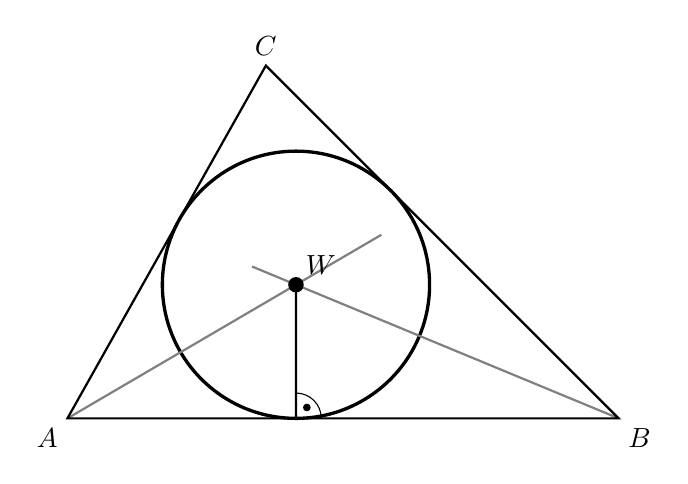
\begin{tikzpicture}[scale=1.4]
  \coordinate (A) at (0,0); \coordinate (B) at (5,0); \coordinate (C) at (1.8,3.2); \coordinate (W) at (2.073,1.212);
  \draw[very thick] (W) circle (1.212);
  \draw[gray, thick] (A) -- (30.32:3.3);
  \draw[gray, thick] (B) -- ++(157.5:3.6);
  \draw[thick] (W) -- (2.073,0);
  \draw (2.073,0) ++(0.23,0) arc (0:90:0.23); \fill (2.073,0) ++(45:0.14) circle (1pt);
  \draw[thick] (A) -- (B) -- (C) -- cycle;
  \fill (W) circle (2pt) node[above right] {$W$};
  \node[below left] at (A) {$A$}; \node[below right] at (B) {$B$}; \node[above] at (C) {$C$};
\end{tikzpicture}}

\vspace{1cm}

{\Large\bfseries Aufgaben im Heft\par}
\medskip
Buch S.\,\rule{1.5cm}{0.4pt} Nr.\,\rule{5cm}{0.4pt}

\kaestchen
\end{document}
